\documentclass{article}

\usepackage{color,amsmath,amssymb,graphicx,fancyhdr,amsfonts,amsthm,verbatim,bbold,environ}
\usepackage{hyperref}
\usepackage{mkolar_definitions}
\usepackage{multirow}
\usepackage{diagbox}
\usepackage{longtable,booktabs}
\usepackage[usenames]{xcolor}
\usepackage[left=2cm,top=2cm,right=2cm,bottom=3cm]{geometry}
% \numberwithin{algorithm}{section}

\newcommand{\tightlist}{%
  \setlength{\itemsep}{0pt}\setlength{\parskip}{0pt}}


%%%%%%%%%%%%%%%%%%%%%%%%%%%%%
\newcommand{\tta}{\theta}
\newcommand{\lag}{\left\langle}
\newcommand{\rag}{\right\rangle}
\newcommand{\lnorm}{\left\|}
\newcommand{\rnorm}{\right\|}
%%%%%%%%%%%%%%%%%%%%%%%%%%%%%
\setlength{\lineskip}{0.25em} 
\setlength{\parskip}{0.5em} 
\usepackage[ruled,lined,boxed,linesnumbered]{algorithm2e}


\title{CS222 Algorithm Design and Analysis  Homework 7}
\author{Zhou Litao 518030910407 F1803016}
\date{\today , Fall Semester}
\begin{document}
\maketitle

%%%%%%%%%%%%%%%%%%%%%%%%%%%%%%%%%%%%%%%%%%
%%%%%%%%%%%%%                 %%%%%%%%%%%%
%%%%%%%%%%%%%    EXERCISE 1   %%%%%%%%%%%%
%%%%%%%%%%%%%                 %%%%%%%%%%%%
%%%%%%%%%%%%%%%%%%%%%%%%%%%%%%%%%%%%%%%%%%
\begin{exercise}[]{
    Provide three programming examples in which multithreading provides better performance than a single-threaded solution.}
  \begin{solution}
  \par{~}
  \begin{enumerate}
      \item In Matrix Multiplication, matrix can be tiled to execute block multiplication within different threads, so that the computation can be accelerated in parallel.
      \item In services that are related to communication between users, multithreading can help the server handle multiple requests at the same time, so that one user's request won't be easily blocked by others if error occurs.
      \item In modern AI applications, models that require massive computation such as neutral networks have taken multithreading into popular use, in order to make sure that multiple data can be processed at the same time to make the AI system efficient.
  \end{enumerate}
  \end{solution}
  \label{ex1}
\end{exercise}

%%%%%%%%%%%%%%%%%%%%%%%%%%%%%%%%%%%%%%%%%%
%%%%%%%%%%%%%                 %%%%%%%%%%%%
%%%%%%%%%%%%%    EXERCISE 2   %%%%%%%%%%%%
%%%%%%%%%%%%%                 %%%%%%%%%%%%
%%%%%%%%%%%%%%%%%%%%%%%%%%%%%%%%%%%%%%%%%%
\begin{exercise}[]{Consider the following code segment:
    \begin{verbatim}
        pid_t pid;
        pid = fork();
        if (pid == 0) { /* child process */
             fork();
             thread_create(. . .);
        }
        fork();
    \end{verbatim}
    \begin{enumerate}
        \item [1)]
        How many unique processes are created?
        \item [2)]
        How many unique threads are created?
    \end{enumerate}
    }
  \begin{solution}
  \par{~}
  \begin{enumerate}
      \item In addition to the main process, 5 new processes are created.
      \item 2 new threads are created.
  \end{enumerate}
  My experiment result can be found below.
  \begin{figure}[h]
    \begin{center}
        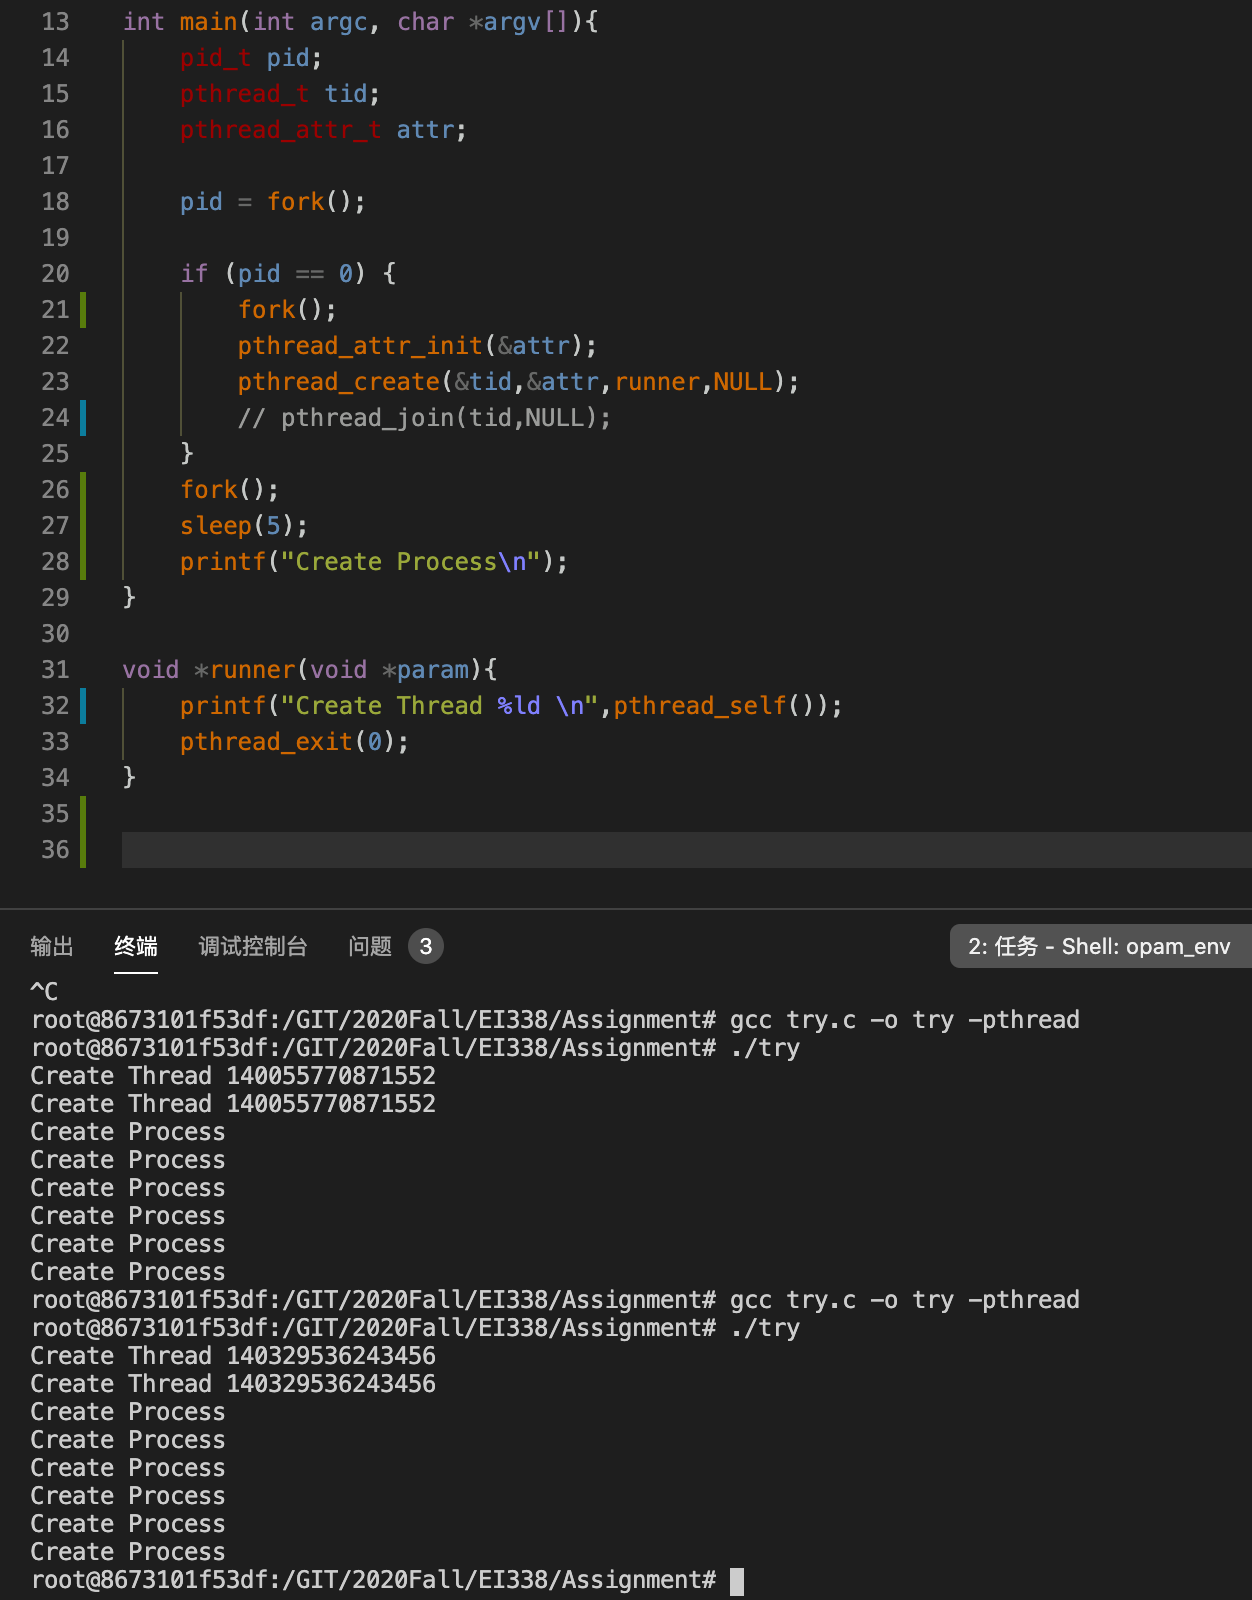
\includegraphics[scale=0.6]{ex7.png}
    \end{center}
    \end{figure}
  \end{solution}
  \label{ex2}
\end{exercise}




%%%%%%%%%%%%%%%%%%%%%%%%%%%%%%%%%%%%%%%%%%
%%%%%%%%%%%%%                 %%%%%%%%%%%%
%%%%%%%%%%%%%    EXERCISE 3   %%%%%%%%%%%%
%%%%%%%%%%%%%                 %%%%%%%%%%%%
%%%%%%%%%%%%%%%%%%%%%%%%%%%%%%%%%%%%%%%%%%
\begin{exercise}[]{The program shown in below uses the Pthreads API. What would be the output from the program at LINE C and LINE P?   
    \begin{figure}[t]
        \begin{center}
            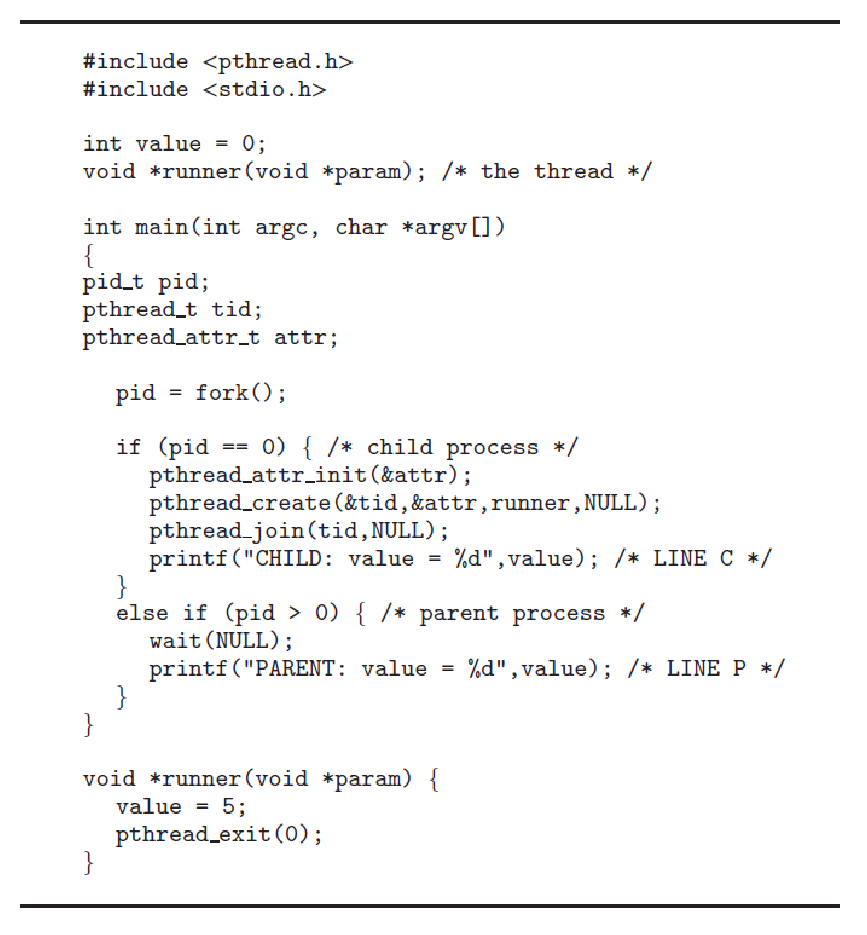
\includegraphics[scale=0.8]{aa1.pdf}
        \end{center}
    \end{figure}}
  \begin{solution}
  \par{~}
  \begin{enumerate}
      \item Line C outputs 5
      \item Line P outputs 0
  \end{enumerate}
  \end{solution}
  \label{ex3}
\end{exercise}




\end{document}